\section{Physical problem and energetic measures}
\label{sec:formulation}

\subsection{Geometry and parameter ranges}
\label{subsec:geometry}

Figure~\ref{fig:geometry} shows the computational domain and its geometric parameters. The domain is a square enclosure of width $L=2a$ and height $H$ with $a=b=0.5$ and $H=1$. The top wall (lid) translates with constant velocity $U_{\mathrm{lid}}$ in the positive $x$-direction; the side walls are stationary. The bottom boundary is the curve
\begin{equation}
y_b(x)= b\left[1-\left(1-\left|\tfrac{x}{a}\right|^{n}\right)^{1/n}\right]
\;+\;\frac{\alpha}{2}\left[1-\cos\!\left(\frac{2\pi N_w (x+a)}{2a}\right)\right],
\label{eq:yb}
\end{equation}
where $x$ is measured from the centre of the domain, $n$ is the superellipse exponent, and $\alpha=h/L$ is the relative undulation amplitude with $N_w$ the number of undulations. The first term is the superelliptic relief; the second is the single-period undulation. For $n=2$ the relief is a semicircle of radius $L/2$ that dips to zero at the centre and rises to mid-height at the corners, giving the smallest fluid area ($A_f=0.893$ at $\alpha=0$). As $n$ increases the relief flattens toward a square bottom, and $A_f$ increases toward $1$ ($A_f=0.989$ at $n=8$, $\alpha=0$). The number of undulations is fixed at $N_w=1$ for all cases reported here, so the transitions $n=2\rightarrow4\rightarrow6\rightarrow8$ isolate the effect of the superellipse exponent at fixed undulation count.

The parameters that vary across the matched contrasts are the superellipse exponent $n\in\{2,4,6,8\}$ and the undulation amplitude $\alpha\in\{0,0.1\}$. The fluid area $A_f$ increases with $n$ at fixed $\alpha$ (Table~\ref{tab:geometry}); it also decreases with $\alpha$. Both effects must be accounted for when interpreting the energetic contrasts, and an area-based reference is introduced in Section~\ref{subsec:area} for this purpose.

\begin{figure}[t]
\centering
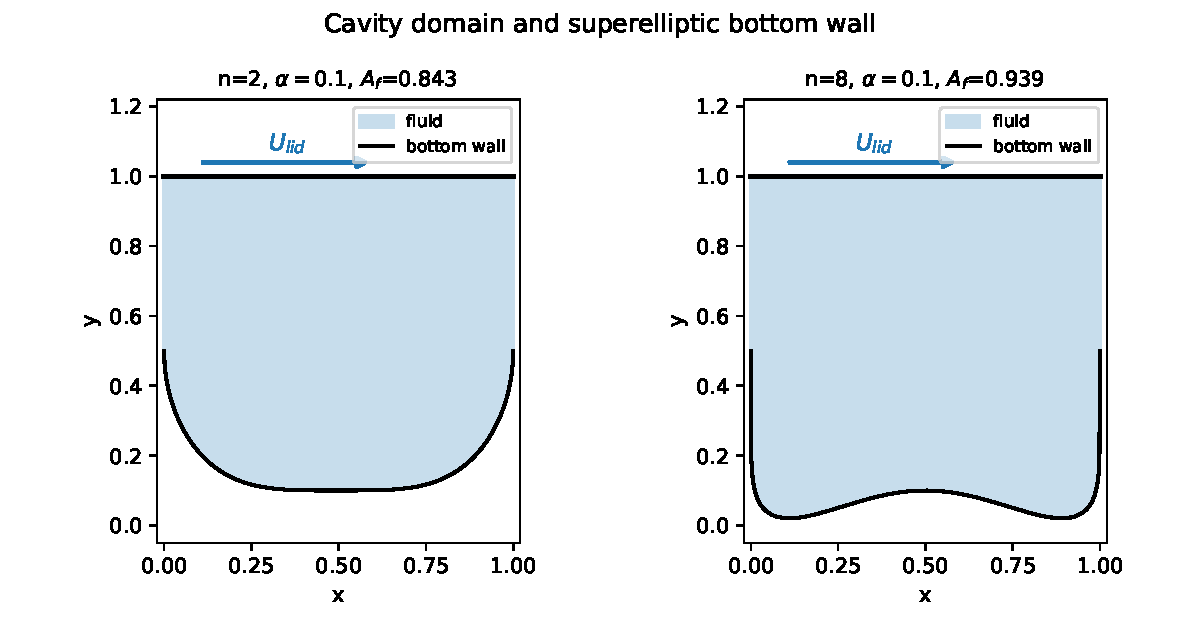
\includegraphics[width=0.85\columnwidth]{figures/fig1_geometry.pdf}
\caption{(Color online) Schematic of the lid-driven cavity with controlled bottom-wall geometry. The domain is a square enclosure of width $L$ and nominal height $L$. The top wall (lid) moves with constant velocity $U_{\mathrm{lid}}$. The bottom boundary follows a superelliptic profile with exponent $n$ and relative undulation amplitude $\alpha = h/L$. The fluid area is $A_f$ (shaded). The three bottom shapes illustrate $n=2$, $n=4$, and $n=8$ at $\alpha=0.1$; the corresponding $\alpha=0$ cases have $\alpha=0$ and are omitted here for clarity.}
\label{fig:geometry}
\end{figure}

\begin{table}[t]
\centering
\caption{Configuration matrix. The bottom wall follows the superelliptic profile of Eq.~\eqref{eq:yb}. The fluid area $A_f$ increases with $n$ toward the square-cavity value $A_f=1$.}
\label{tab:geometry}
\begin{tabular}{@{}ll@{}}
\hline
Parameter & Values \\
\hline
Reynolds number, $Re$ & $100$, $400$, $1000$ \\
Superellipse exponent, $n$ & $2$, $4$, $6$, $8$ \\
Relative undulation amplitude, $\alpha$ & $0$, $0.1$ \\
Grid resolution, $N$ & $128$, $256$, $384$ \\
Number of undulations, $N_w$ & $1$ \\
Semi-axes, $a=b$ & $0.5$ \\
Nominal cavity height, $H$ & $1$ \\
Lid velocity, $U_{\mathrm{lid}}$ & $1$ (unit) \\
\hline
Fluid area, $A_f$ ($\alpha=0$) & $0.8927$ ($n{=}2$), $0.9635$ ($n{=}4$), $0.9819$ ($n{=}6$), $0.9892$ ($n{=}8$) \\
Fluid area, $A_f$ ($\alpha=0.1$) & $0.8427$ ($n{=}2$), $0.9135$ ($n{=}4$), $0.9319$ ($n{=}6$), $0.9392$ ($n{=}8$) \\
\hline
\end{tabular}
\end{table}


\subsection{Governing equations and dimensionless groups}
\label{subsec:governing}

The flow is governed by the incompressible Navier--Stokes equations. In dimensionless form, with lengths scaled by $L$, velocities by $U_{\mathrm{lid}}$, and time by $L/U_{\mathrm{lid}}$, these read
\begin{equation}
\frac{\partial \mathbf{u}}{\partial t} + \mathbf{u}\cdot\nabla\mathbf{u} = -\nabla p + \frac{1}{Re}\nabla^2\mathbf{u}, \qquad \nabla\cdot\mathbf{u}=0,
\label{eq:NS}
\end{equation}
where the Reynolds number is $Re = U_{\mathrm{lid}} L/\nu$ and $\nu$ is the kinematic viscosity. The LBM models this incompressible system at low Mach number; the lattice Mach number $Ma = U/c_s$ (with $c_s$ the lattice sound speed) is $0.06$ or below on the production grid, but rises to about $0.09$ at $N=256$ and $0.18$ at $N=128$ for the higher Reynolds numbers because the lattice speed follows a diffusive scaling (Section~\ref{sec:numerical}). Compressibility effects are therefore small at the resolutions that support the final results but not negligible on the coarse grids, which is one reason those grids are used only for the resolution test.

\subsection{Boundary conditions}
\label{subsec:bc}

The moving lid is prescribed with a regularized velocity profile: the lid velocity is constant across the bulk of the top wall and is smoothed near the two top corners using a smoothstep with transition parameter $\varepsilon=0.02$, reducing the singularity at the corners. The side walls and the curved bottom wall satisfy the no-slip condition via interpolated bounce-back, described in Section~\ref{sec:numerical}. The distinction between physical boundary conditions and their discrete lattice realization is discussed separately below.

\subsection{Energetic measures}
\label{subsec:energetics}

Three volume-integrated quantities are computed for every converged run.

\paragraph{Power input.}
The mechanical power supplied by the moving lid is
\begin{equation}
P = \int_{\Gamma_{\mathrm{lid}}} \mathbf{u}_w \cdot (\boldsymbol{\sigma}\cdot\mathbf{n})\, dS,
\end{equation}
where $\boldsymbol{\sigma}$ is the stress tensor, $\mathbf{n}$ the outward normal, and $\mathbf{u}_w$ the lid velocity. In the LBM implementation, $P$ is extracted directly from the momentum exchange at the lid links, which corresponds to the discrete counterpart of this integral.

\paragraph{Viscous dissipation.}
For a Newtonian incompressible fluid, the total viscous dissipation is
\begin{equation}
D = 2\mu \int_{\Omega} \mathbf{S}:\mathbf{S}\, d\Omega, \qquad
\mathbf{S} = \tfrac{1}{2}\left(\nabla\mathbf{u} + (\nabla\mathbf{u})^{\mathsf{T}}\right),
\end{equation}
with $\mu$ the dynamic viscosity and $\Omega$ the fluid domain. The velocity gradients are computed from the lattice distribution functions using central differences on the grid. The domain is two-dimensional with unit depth.

\paragraph{Kinetic energy.}
The volume-integrated kinetic energy is
\begin{equation}
K = \frac{1}{2}\int_{\Omega} |\mathbf{u}|^2\, d\Omega.
\end{equation}

All three quantities are reported in dimensionless form ($P^*,D^*,K^*$) using the scaling defined in Section~\ref{sec:numerical}. The dimensionless groups are formed from $U_{\mathrm{lid}}$ and $L$ as reference scales.

\paragraph{Independence of the energetic measures.}
For the steady incompressible flow considered here, the kinetic energy is constant in time, so the global mechanical energy balance requires the power input to equal the viscous dissipation, $P=D$. The two quantities $P$ and $D$ are therefore \emph{not} independent observables: they are two discrete estimators of the same physical quantity, and the small residual $|P^*-D^*|/D^*$ reported in Section~\ref{sec:results} (a signed defect that is negative in every case and decays as a first-order-in-$1/N$ discretisation error) measures the difference between the two estimators rather than a physical energy imbalance. Consequently, the only genuinely independent second observable besides the dissipation is the kinetic energy $K^*$; the contrast $I_D$ and the power-based contrast $I_P$ are two routes to the same geometric response, and their agreement (Section~\ref{subsec:consistency}) is a consistency check, not an independent confirmation of a distinct effect. This is why the analysis is built on $I_D$ and uses $I_P$ only as a cross-check.

\subsection{Matched geometric contrasts}
\label{subsec:contrasts}

Let $q$ denote the geometric exponent, taking values $q=2,4,6,8$. For any energetic quantity $Q^*$, the matched contrast between two exponents is defined with a fixed sign convention:
\begin{equation}
I_Q(q_i,q_j) = Q^*(q_j) - Q^*(q_i), \qquad i<j.
\label{eq:contrast}
\end{equation}
The three contrasts studied are $I_Q(2,4)$, $I_Q(4,6)$, and $I_Q(6,8)$. A positive $I_D$ means that the higher-exponent geometry dissipates more energy than the lower-exponent one, under this convention. These contrasts are \emph{differences} between paired simulations, not absolute power or dissipation values; a large relative variation of a small absolute contrast must be interpreted with care, as discussed in Section~\ref{sec:results}.

Note that the estimator discrepancy $\delta_{IP/ID}$ of Section~\ref{subsec:consistency} measures the agreement between two discrete estimators of the same physical quantity; it is distinct from, and must not be confused with, the resolution uncertainty of $I_D$ itself, which is quantified in Section~\ref{subsec:robustness}.

Unless stated otherwise, contrasts are quoted as percentages of the earlier configuration of the pair,
\begin{equation}
I_Q(q_i,q_j)=\frac{Q^*(q_j)-Q^*(q_i)}{Q^*(q_i)}\times 100\%,
\end{equation}
so that the denominator is always $D^*(q_i)$ or $P^*(q_i)$ and the sign follows the numerator.

\subsection{Area-based reference model}
\label{subsec:area}

The fluid area is \emph{not} constant across the exponent transitions: increasing $n$ flattens the bottom wall toward the square-cavity limit $A_f=1$ (Table~\ref{tab:geometry}). A null hypothesis is therefore tested: that the change in dissipation across a geometric transition is fully explained by the change in fluid area, i.e.\ that the dissipation is extensive in the fluid amount. Under this hypothesis the dissipation would scale with $A_f$, and the predicted contrast would be
\begin{equation}
I_{D,\mathrm{area}}(q_i,q_j) = \left(\frac{A_f(q_j)}{A_f(q_i)} - 1\right)\times 100\%.
\label{eq:area}
\end{equation}
Since $A_f$ increases from $0.8927$ ($n=2$) to $0.9635$ ($n=4$), this extensive reference predicts a contrast of $+7.93\%$ for the transition $(2,4)$. The comparison with the measured $I_D$ in Section~\ref{subsec:arearesult} quantifies how far the actual response is from this extensive limit.
\subsection{Non-additivity and interaction}
\label{subsec:interaction}

If an interaction between the superellipse exponent and the undulation amplitude is to be claimed, it must be defined as a difference of differences, not inferred from a fitted model. For amplitude values $\alpha_1$ and $\alpha_0$,
\begin{equation}
\mathcal{I}_Q = \left[Q^*(q_j,\alpha_1)-Q^*(q_i,\alpha_1)\right] - \left[Q^*(q_j,\alpha_0)-Q^*(q_i,\alpha_0)\right].
\end{equation}
This quantity is reported when both amplitude values are available; otherwise, the discussion is restricted to the matched contrasts at fixed amplitude. With only two amplitude levels ($\alpha\in\{0,0.1\}$), $\mathcal{I}_Q$ is a single finite difference and cannot by itself establish a functional dependence on $\alpha$; it establishes only that the contrast \emph{changes} with amplitude. We therefore use $\mathcal{I}_Q$ strictly as a difference-of-differences estimator and refrain from any statement about the form of an interaction law.




